\section{System description}
\label{sec:Description}

\subsection{Overview}

\noindent The working principle of the L1 tracking system is sketched on Fig.~\ref{fig:L1TT_principle}. Relevant tracker information is retrieved by the track trigger board where it is handled by a data organization unit (DO), which extract the info necessary to the pattern recognition (PR) and send it to the PR unit. There PR is performed using dedicated associative memory chip (AM). 

\begin{figure}[ht!]
\centering
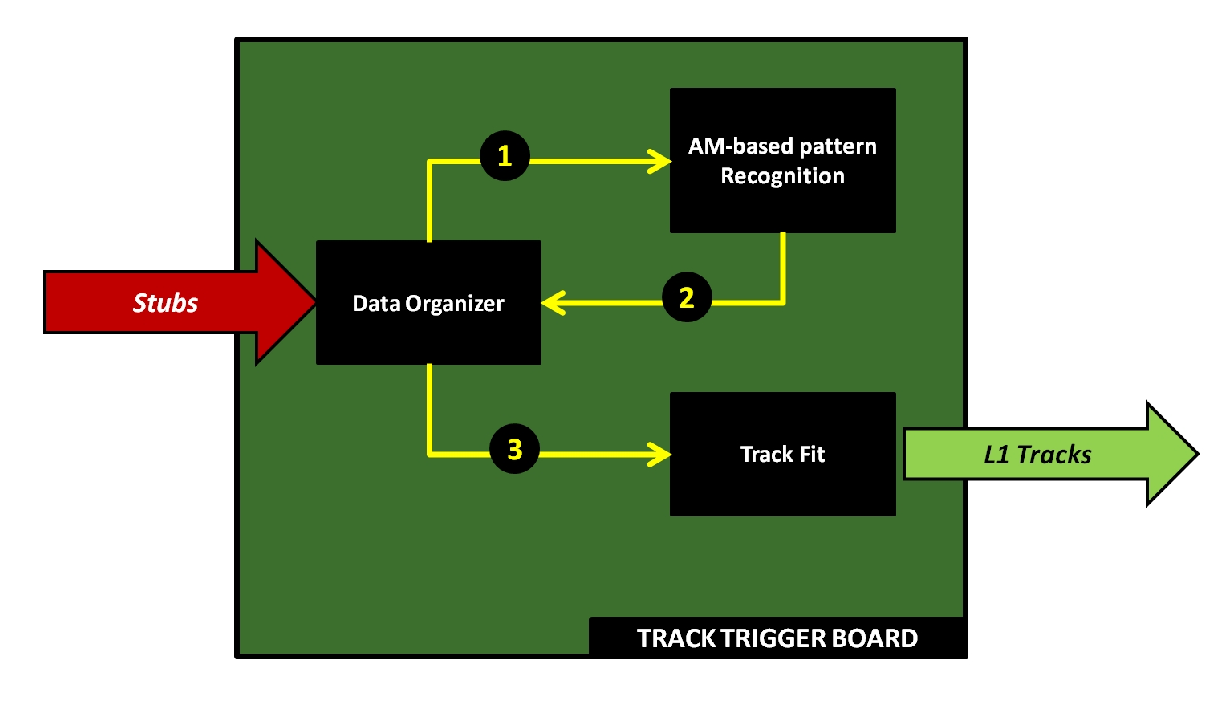
\includegraphics[width=0.7\columnwidth]{Plots/L1TTprin.eps}
\caption{L1 tracking principle}
\label{fig:L1TT_principle}
\end{figure}

\noindent The track candidate (patterns) are sent back to the DO unit, where the corresponding hits are retrieved and sent to the track fit unit (TF). This unit computes the track parameters and send them to the L1 central trigger board, where they are mixed with the information of the other subdetectors. From this one understand that the total latency available for track reconstruction is only a fraction of the overall L1 latency. The current recommendation being $10~\mu s$, we based our developments on $\approx 6\mu s$ for the whole tracking stage.

\subsection{Data flow}

\noindent The way L1 tracking trigger enters the CMS dataflow is presented in Fig.~\ref{fig:L1TTinteg}. The data is extracted from the tracker and sent to the front-end drivers (FED). The L1 tracking problem begins here. 

\begin{figure}[ht!]
\centering
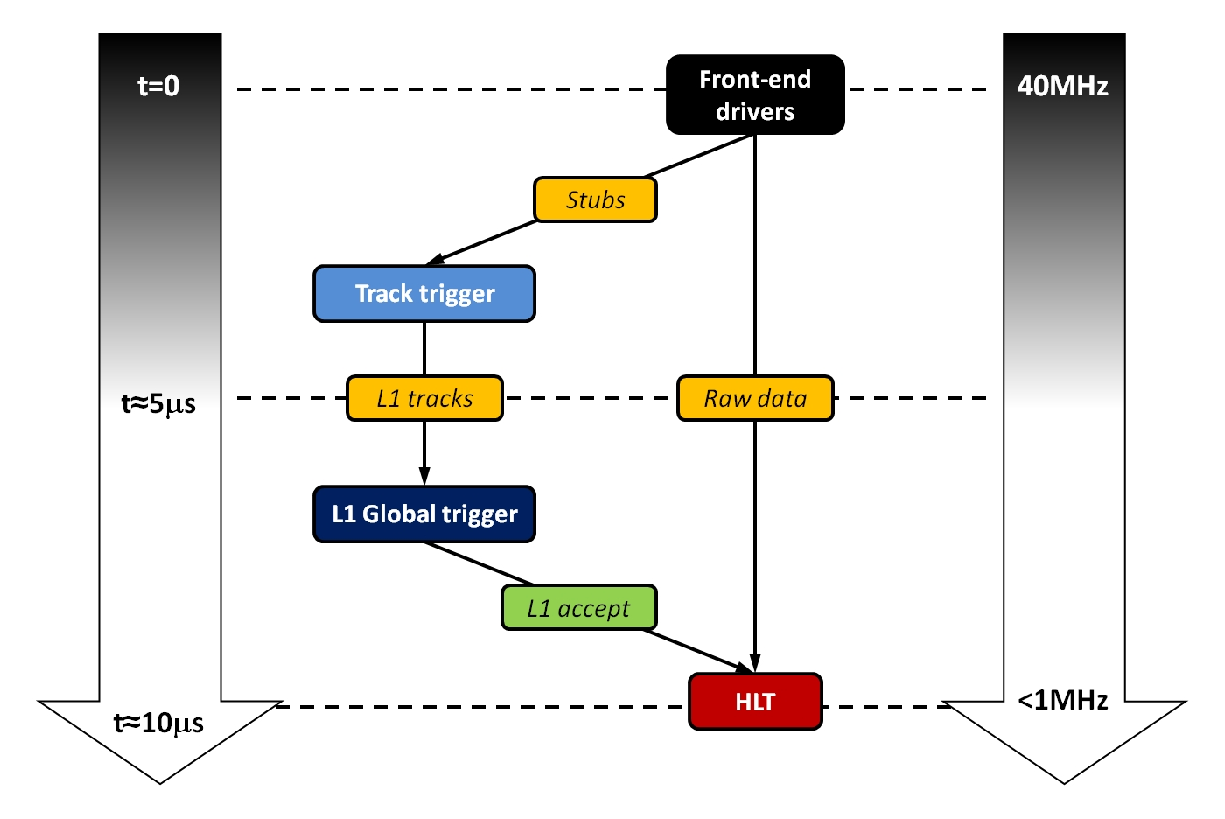
\includegraphics[width=0.6\columnwidth]{Plots/TTintegration.eps}
\caption{\emph{Track trigger within the CMS dataflow}}
\label{fig:L1TTinteg}
\end{figure}

\noindent The Phase II tracker FEDs will have two outputs links. The first link will send raw data to a pipeline where it will wait for the L1 accept signal (this is what happens currently in CMS), whereas the second will provide skimmed information (Stubs) to the track trigger boards. This data is sent to the track trigger boards at a $40~MHz$ rate. 

\noindent In addition, the track trigger system has to provide the track information for each event. The whole system should thus be able to sustain an output rate of $40~MHz$. The information sent to the central L1 trigger system (L1GT) consists in a list of track parameters ($p_T$,$\phi$,$z_0$,$\eta$,quality flag,...). The way this info is used is the responsibility of the L1GT, and is therefore not discussed in this document. 

\subsection{Interface with Tracker FEDs and L1 Global Trigger}

\noindent As we will see in Section~\ref{sec:Hardware}, bringing the information from the FEDs to the track trigger boards will be a critical point of this project. Of course one can not fit process the whole tracker data with one single track trigger boards. Therefore the tracker will be divided into overlapping trigger sectors. Each sector will cover a certain range in $\eta$ and $\phi$ direction, and will have to satisfy L1 track trigger system requirements ($p_T$ threshold, maximum rate,...). Each track trigger board will reconstruct tracking information for one sector, it therefore will have to receive the data contained in this sector. The method we plan to use to do that is sketched on Figure~\ref{fig:L1TTmap}: 

\begin{figure}[ht!]
\centering
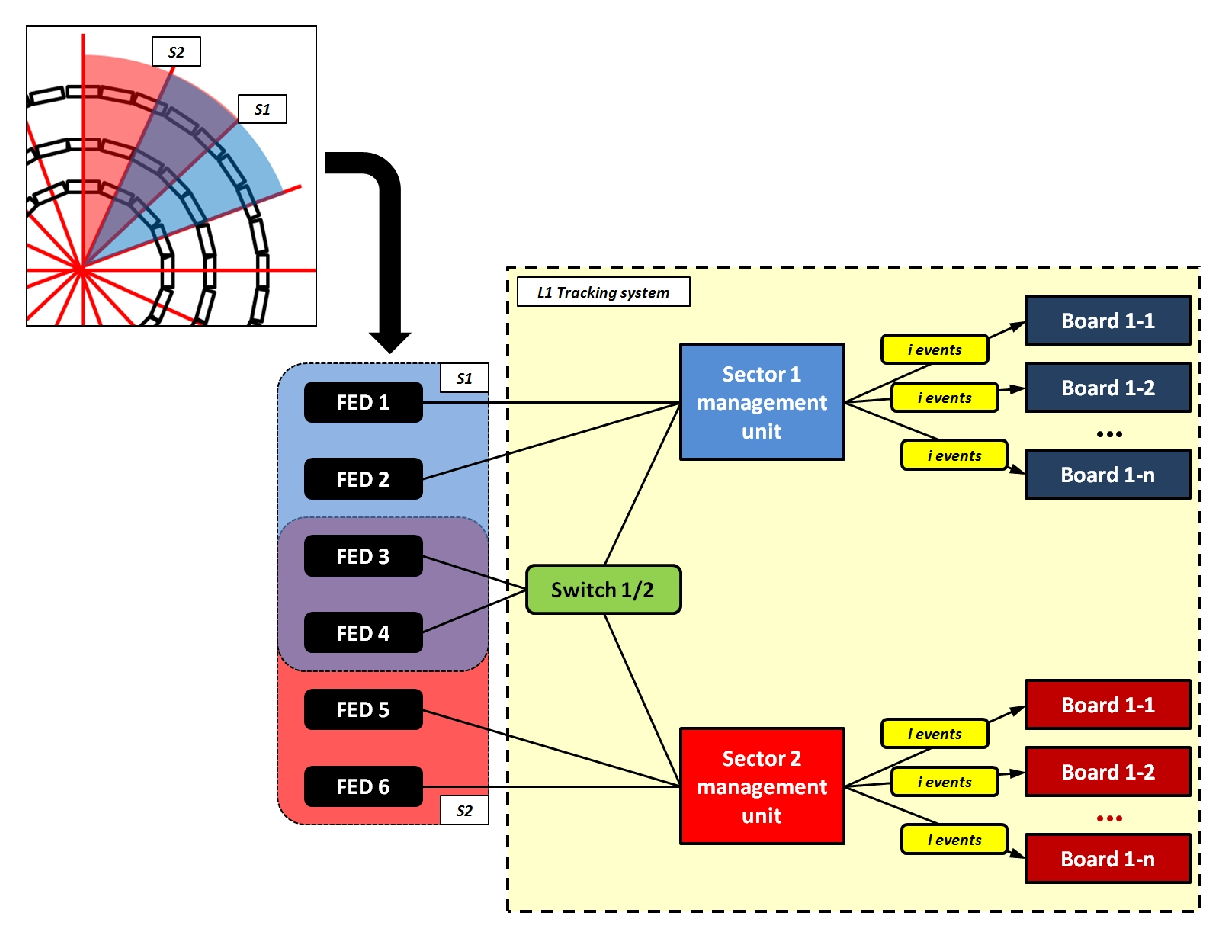
\includegraphics[width=0.7\columnwidth]{Plots/TTmapping.eps}
\caption{\emph{Bringing FED data to track trigger boards.}}
\label{fig:L1TTmap}
\end{figure}

\noindent On this figure one deals with only two sectors, but the idea is the same for the whole tracker. Each FED will contain the data from a certain number of sectors. In our example, FED 1 contains only information from sector 1, whereas FED 3 is in an overlapping region, and thus contains info for sectors 1 and 2. FED 1 data can be transmitted directly to sector 1 management unit, whereas FED 3 data has to be duplicated into one switching board sending data to sectors 1 and 2. All the FEDs in the same situation can use the same switching unit, there is therefore only a limited number of switching units required.

\noindent After this step, the data reaches a sector management unit (SMU), which just send the event information to a free sector trigger board. One event will arrive in the SMU every $25~ns$, therefore events will have to be processed in parallel in order to sustain this rate. The number of boards necessary for each sector clearly depends on the latency of the different tracking steps within a boards. This point will be discussed in more details in Part~\ref{sec:Hardware}.

\noindent Providing the track parameters to the L1GT unit is a less complex procedure. The amount of data to transmit will indeed be much smaller than at the entrance of the system. However, as many events will be treated in parallel in independent sectors, one will have to take of data retrieval before its transmission to L1.

\subsection{Simulation tools and needs}


\clearpage
